\documentclass[10pt,colorlinks]{beamer}
  % compress
  %\documentclass[handout,xcolot=pdftex,dvipsnames,table]{beamer}
\definecolor{mybg}{RGB}{255,255,204}
\usepackage{minted}
\usepackage{graphicx}
\usepackage[english]{babel}
\usepackage[utf8x]{inputenc}
\usepackage{amsmath}


 \usepackage{beamerthemesplit}

%\usemintedstyle{trac}

\mode<presentation>
\setbeamercovered{invisible}
\usetheme{Warsaw}
\usecolortheme{dolphin}

\usefonttheme{serif}







% Delete this, if you do not want the table of contents to pop up at
% the beginning of each subsection:
\AtBeginSection[]
{
  \begin{frame}<beamer,allowframebreaks>{Outline}
    \tableofcontents[currentsection]
  \end{frame}
}



\title{ Python para RPi}
\subtitle
{Parte II: Introducción a Python} % (optional)


\author[Velasco and Perera]{Manel Velasco,\inst{1} PhD and Alexandre Perera,\inst{1}$^{,}$\inst{2} PhD}

\institute[UPC] % (optional, but mostly needed)
{
  \inst{1}%
  Departament d'Enginyeria de Sistemes, Automatica i Informatica Industrial (ESAII)  \\
  Universitat Politecnica de Catalunya 
  \and 
  \inst{2}%
   Centro de Investigacion Biomedica en Red en Bioingenieria, Biomateriales y Nanomedicina (CIBER-BBN)  \\
    \href{mailto:Alexandre.Perera@upc.edu}{Alexandre.Perera@upc.edu}~\href{mailto:manel.velasco@upc.edu}{Manel.Velasco@upc.edu}
}
 

\date[Feb, 2013, Learning Python]{Introduction to Python for Engineering and Statistics\\
Febraury, 2013}

 %

\begin{document}


\begin{frame}[plain]
   %  \titlepage
   \maketitle
\end{frame}


\begin{frame}[allowframebreaks]{Contents}
  \tableofcontents
  % You might wish to add the option [pausesections]
 \note[options]{aixo son notes}
\end{frame}

\section{Introducción}

%----------------------------FRAME 2 cols------------------------------
\begin{frame}[fragile]\frametitle{¿Que es Python?}
Hola
\end{frame}

%----------------------------FRAME------------------------------------
\begin{frame}[fragile]\frametitle{Ejemplo}
este es un ejemplo
\end{frame}

%----------------------------FRAME------------------------------------
\begin{frame}[fragile]\frametitle{Why not?}
 \begin{itemize}
    \item ¿Python?¿Python?¿Python?¿Python?
        \begin{itemize}
            \item Ventajas:
                \begin{itemize}
                     \item \tiny Muchas librerias científicas en el mercado
                    \item \tiny Lenguaje bien pensado desde un principio, muy facil de leer y bien estructurado, "Codificamos lo que pensamos".
                    \item \tiny Muchas librerias para aspectos no relacionados con la ciencia (servidores web, captura de imágenes...)
                    \item \tiny Libre y abierto, muy extendido y con una comunidad muy activa.
                \end{itemize}
            \item Desventajas:
                \begin{itemize}
                    \item \tiny Los entornos de desarrollo son menos placenteros que en otros lenguajes.
                    \item \tiny Desde un punto de vista científico no es posible encontrar todos los algoritmos implemenetados. 
                \end{itemize}
        \end{itemize}
\end{itemize}
\begin{block}{\begin{center}
    No es obligatorio
\end{center}}
\begin{center}
No hace falta usar Python... pero...,\\ \textbf{No pasa nada por intentarlo}\end{center}
\end{block}


\end{frame}

%----------------------------FRAME------------------------------------
\begin{frame}[fragile]\frametitle{Historia}
\begin{columns}[T]
    \begin{column}{.7\textwidth}
        \begin{block}{\centering Historia}
\small
            \begin{itemize}
                 \item Python 1.0 - Enero 1994
                    \begin{itemize}
\tiny
                        \item Python 1.5 - Diciembre 31, 1997
                        \item Python 1.6 - Septiembre 5, 2000
                    \end{itemize}
                \item Python 2.0 - Octubre 16, 2000
                    \begin{itemize}
\tiny
                        \item Python 2.1 - Abril 17, 2001
                        \item Python 2.2 - Diciembre 21, 2001
                        \item Python 2.3 - Julio 29, 2003
                        \item Python 2.4 - Noviembre 30, 2004
                        \item Python 2.5 - Septiembre 19, 2006
                        \item Python 2.6 - Octubre 1, 2008
                        \item \textbf{Python 2.7 - Julio 3, 2010}
                    \end{itemize}
                \item Python 3.0 - Diciembre 3, 2008
                    \begin{itemize}
\tiny
                        \item Python 3.1 - Junio 27, 2009
                        \item Python 3.2 - Febrero 20, 2011
                        \item Python 3.3 - Septiembre 29, 2012
                    \end{itemize}
            \end{itemize}
        \end{block}
    \end{column}
    \begin{column}{.3\textwidth}
        \begin{block}{ \centering  Guido van Rossum}
            \begin{center}
                Pensado al final de los 80s por 
                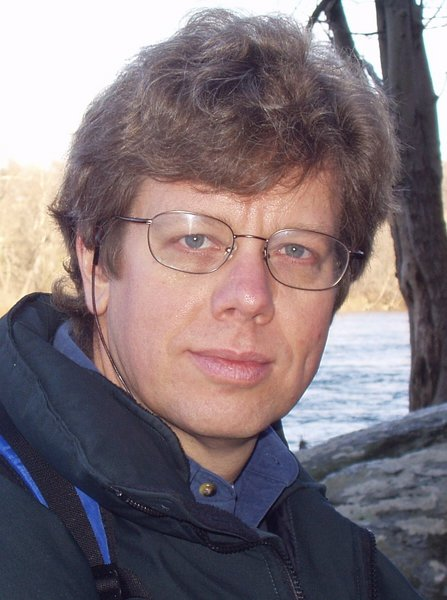
\includegraphics[scale=0.2]{figs/Guido_van_Rossum.jpg}
            \end{center}
        \end{block}
    \end{column}
  \end{columns}
\end{frame}

%----------------------------FRAME------------------------------------
\begin{frame}[fragile]\frametitle{Installation}

  \begin{columns}[T]
    \begin{column}{.4\textwidth}
        \begin{block}{\centering Linux}
\begin{center}
    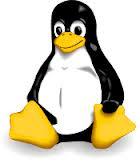
\includegraphics[scale=0.3]{figs/linux.jpg}
\end{center}
                  apt-get install python
        \end{block}
    \end{column}
    \begin{column}{.6\textwidth}
        \begin{block}{ \centering  Windows}
\centering

\begin{center}

\includegraphics[scale=0.3]{figs/windows.jpg}
\end{center}    
            Ir a \textbf{http://www.python.org/getit/}
            y descargar 
\textbf{Python 2.7.3 Windows Installer}
        \end{block}        
    \end{column}
  \end{columns}
\end{frame}

\subsection{Python Resources}
%----------------------------FRAME------------------------------------
\begin{frame}[fragile]\frametitle{Resources}
\begin{block}{AYUUUUUUUUDDDAAAAAAA!!!}
\textbf{http://python.org}
\begin{center}
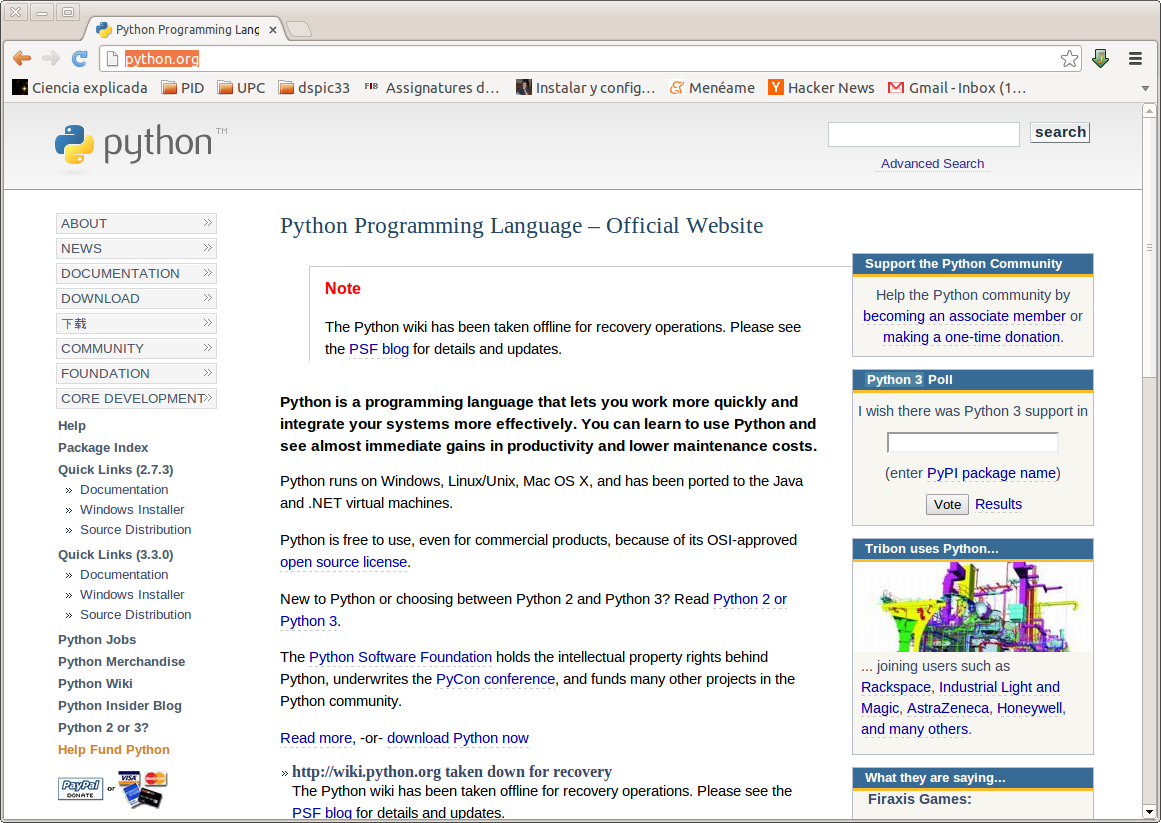
\includegraphics[scale=0.15]{figs/python__org.jpg}
\end{center}  
\end{block}
  
\end{frame}

%-------------------------------------------------------------------
%---------------------------SECTION---------------------------------
%-------------------------------------------------------------------

\section{Trabajando con Python}

\subsection{Modods de trabajar}

%----------------------------FRAME------------------------------------
{
\usebackgroundtemplate{
  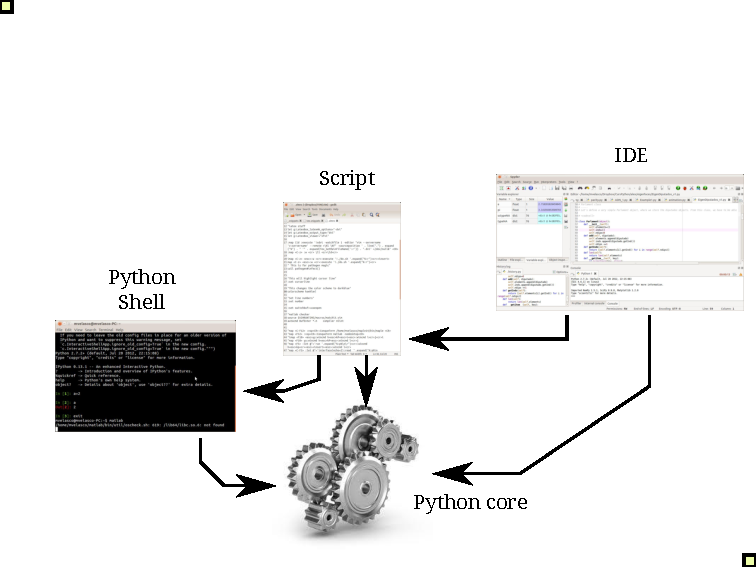
\includegraphics[width=\paperwidth,height=\paperheight]{figs/workflow.pdf}
}

\begin{frame}[fragile]\frametitle{Modos de trabajar}
\end{frame}
}
%----------------------------FRAME------------------------------------
\begin{frame}[fragile]\frametitle{El intérprete Python}
 
 \begin{columns}[T]
    \begin{column}{.7\textwidth}
        \begin{block}{\centering El intérprete Python}
\small Python es abierto, es una especificación, por lo tanto hay muchas implementaciones de Python:
\begin{description}
\scriptsize    
    \item[CPython] Implementación or defecto (C, C++)
    \item[CLPython] Implementación de Python en Lisp
    \item[Jython] Implementación de Python en Java
    \item[PyPy] La implementación de Python en Python
    \item [IronPython] Implementación en C\# 
\end{description}
        \end{block}
    \end{column}
    \begin{column}{.3\textwidth}
\begin{center}
Intérprete Python
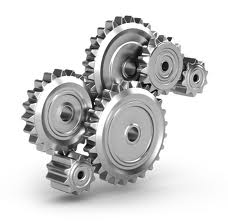
\includegraphics[scale=0.3]{figs/gears.jpg}
\end{center}    
    \end{column}
  \end{columns}
\end{frame}


%----------------------------FRAME------------------------------------
\begin{frame}[fragile]\frametitle{Python Shell}
        \begin{block}{\centering Python Shell}
\small Hay muchas maneras d trabajar directamente con Python, las más destacadas son: 
    \begin{description}
\scriptsize    
        \item[CLIPython] La manaera más sencilla.
        \item[IPython] shell de python mejorada (muy mejorada)
    \end{description}
\end{block}
\begin{figure}
\begin{minipage}[b]{0.45\linewidth}
\centering
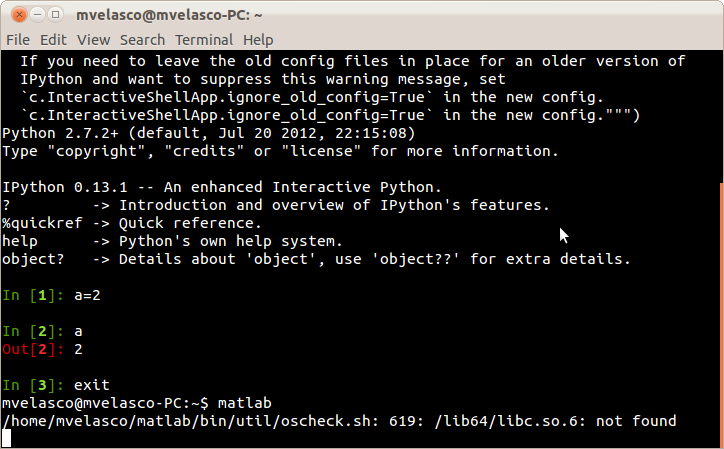
\includegraphics[width=\textwidth]{figs/commandline.jpg}
\end{minipage}
\hspace{0.5cm}
\begin{minipage}[b]{0.45\linewidth}
\centering
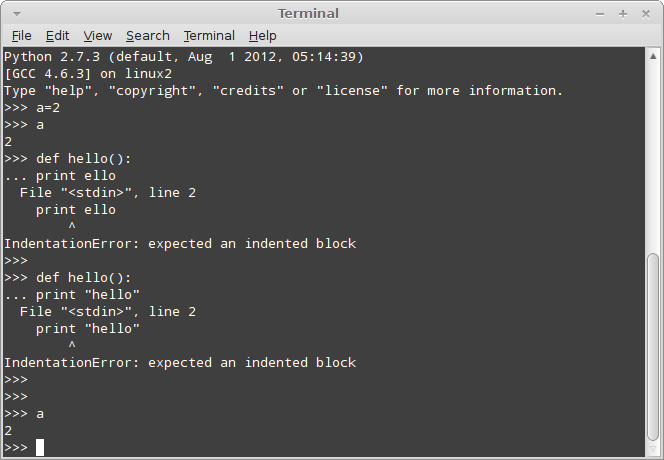
\includegraphics[width=\textwidth]{figs/commandline2.jpg}
\end{minipage}
\end{figure}    
\end{frame}




\subsection{Text Editors} % (fold)
%----------------------------FRAME------------------------------------
\begin{frame}[fragile]\frametitle{Editores de texto}
\begin{block}{Editores de texto}
 Cualquier editor de textos es adecuado para escribir programas en Python, pero recomendamos que tenga algunas características:
\begin{itemize}
    \item Substitución de tabuladores por espacios.
    \item Inserción automática de pedazos de código repetitivos
    \item Autocompletado
\end{itemize}
En el universo Linux, tanto Vim como Emacs tienen estas características.
\end{block}

\end{frame}

\subsection{IDEs}
%----------------------------FRAME------------------------------------
\begin{frame}[fragile]\frametitle{IDEs}
 \begin{block}{Los IDEs más adecuados}
 \begin{description}
     \item[Spyder] Entorno parecido a Matlab, orientado a entornos científicos.
     \item[Eclipse-PyDEV] IDE orientado a grandes proyectos  
 \end{description}
 \end{block}
\begin{center}
    \textbf{DEMO}
\end{center}

\end{frame}










%-------------------------------------------------------------------
%---------------------------SECTION---------------------------------
%-------------------------------------------------------------------


\section{Primeros pasos con Python}

\subsection{Introducción}
%----------------------------FRAME------------------------------------
\begin{frame}[fragile]\frametitle{Primer paso}
\begin{block}{\centering Paso 1}
\centering Abra un intérprete y escriba ... 
\end{block}
  %-------------------------------CODE
\begin{minted}[bgcolor=mybg,frame=lines,mathescape]{python}
>>> print "Hello, world"
Hello, world
\end{minted}

\begin{block}{}
\centering Bienvenido a Python,\\ acaba de ejecutar su primera instrucción en python, felicidades!
\end{block}
%-------------------------------END CODE
\end{frame}

%----------------------------FRAME------------------------------------
\begin{frame}[fragile]\frametitle{Segundo paso}
\vspace{-0.1cm}
\begin{block}{\centering Paso 2}
\centering Para emepezar a sentirnos cómodos en python inroduzca la siguiente ristra de instrucciones en el intérprete
\end{block}
 \begin{columns}[T]
\begin{column}{.5\textwidth}
%-------------------------------CODE
\tiny
\begin{minted}[bgcolor=mybg,frame=lines,mathescape]{python}
>>> a = 3
>>> b = 2*a
>>> type(b)
<type 'int'>
>>> print b
6
>>> a*b
18
>>> b = 'hello'
>>> type(b)
<type 'str'>
>>> b + b
'hellohello'
>>> 2*b
'hellohello'
\end{minted}

%-------------------------------END CODE

\end{column}
    \begin{column}{.5\textwidth}
\end{column}
\end{columns}
\end{frame}

%----------------------------FRAME------------------------------------
\begin{frame}[fragile]\frametitle{Second step}
\vspace{-0.1cm}
\begin{block}{\centering STEP 2}
\centering Para emepezar a sentirnos cómodos en python inroduzca la siguiente ristra de instrucciones en el intérprete
\end{block}
 \begin{columns}[T]
\begin{column}{.5\textwidth}
%-------------------------------CODE
\tiny
\begin{minted}[bgcolor=mybg,frame=lines,mathescape]{python}
>>> a = 3
>>> b = 2*a
>>> type(b)
<type 'int'>
>>> print b
6
>>> a*b
18
>>> b = 'hello'
>>> type(b)
<type 'str'>
>>> b + b
'hellohello'
>>> 2*b
'hellohello'
\end{minted}

%-------------------------------END CODE

\end{column}
    \begin{column}{.5\textwidth}
    \begin{block}{\centering Observe que...}
            \begin{itemize}
\scriptsize    
                \item No declaramos variables (hurra!!!!!) 
                \item El tipo de la variable puede cambiar cuando queramos (hurra!!!, hurra!!!)
                \item Hay una manera de saber cual es el tipo de una variable en un momento dado.
            \end{itemize}
       \end{block}

\end{column}
\end{columns}
\end{frame}

\subsection{Tipos básicos}
%----------------------------FRAME------------------------------------
\begin{frame}[fragile]\frametitle{Types}
 \begin{columns}[T]
\begin{column}{.5\textwidth}
   \begin{block}{Integer}
 %-------------------------------CODE
\tiny
\begin{minted}[bgcolor=mybg,frame=lines,mathescape]{python}
>>> 1+1
2
>>> a=4
\end{minted}

 %-------------------------------END CODE
  \end{block}
 \begin{block}{Boolean}
%-------------------------------CODE
\tiny
\tiny
\begin{minted}[bgcolor=mybg,frame=lines,mathescape]{python}
>>> 3 > 4
False
>>> test = (3 > 4)
>>> test
False
>>> type(test)
<type 'bool'>
\end{minted}

%-------------------------------END CODE
\end{block}
\end{column}
    \begin{column}{.5\textwidth}
 \begin{block}{Float}
%-------------------------------CODE
\tiny
\begin{minted}[bgcolor=mybg,frame=lines,mathescape]{python}
>>> c=2.1
>>> 3.5/c
1.6666666666666665
\end{minted}


%-------------------------------END CODE
\end{block}
  \begin{block}{Complex}
%-------------------------------CODE
\tiny
\begin{minted}[bgcolor=mybg,frame=lines,mathescape]{python}
>>> a=1.5+0.5j
>>> a.real
1.5
>>> a.imag
0.5
>>> import cmath
>>> cmath.phase(a)
0.3217505543966422
\end{minted}

%-------------------------------END CODE  
  \end{block}

\end{column}
\end{columns}
\end{frame}
%----------------------------FRAME------------------------------------
\begin{frame}[fragile]\frametitle{Calculadora Básica}
\begin{block}{Un shell de Python es como una calculadora de bolsillo con las operaciones básicas +, -, *, /, \% (modulo) implementadas de forma nativa:}
%-------------------------------CODE
\begin{minted}[bgcolor=mybg,frame=lines,mathescape]{python}
>>> 7 * 3.
21.0
>>> 2**10
1024
>>> 8 % 3
2
\end{minted}

%-------------------------------END CODE
\end{block}

\end{frame}
%----------------------------FRAME------------------------------------
\begin{frame}[fragile]\frametitle{ATENCIÓN!}
\begin{block}{División entera}
%-------------------------------CODE
\small
\begin{minted}[bgcolor=mybg,frame=lines,mathescape]{python}
>>> 3/2
1
\end{minted}

%-------------------------------END CODE
\end{block}
\begin{block}{Utilice floats}
%-------------------------------CODE
\tiny
\begin{minted}[bgcolor=mybg,frame=lines,mathescape]{python}
>>> 3 / 2.
1.5
>>> a = 3
>>> b = 2
>>> a / b
1
>>> a / float(b)
1.5
\end{minted}

%-------------------------------END CODE
\end{block}
\end{frame}








%----------------------------FRAME------------------------------------
\begin{frame}[fragile]\frametitle{EJERCICIOS BÁSICOS}
\begin{block}{Escriba scripts que resuelvan los siguientes problemas}
\begin{itemize}
    \item ¿Cuál es la diferencia entre usar "+" y "", en un comando de impresión? Pruébelo!
    \item Escriba un programa que pregunte al usuario dos nombres, guarde estos nombres en variables y escriba un saludo a ambos a la vez
\end{itemize}

\end{block}


\end{frame}




%----------------------------FRAME------------------------------------
\begin{frame}[fragile]\frametitle{Listas}
Python proporciona un conjunto de tipos básicos denominados "contenedores" que son muy importantes dentro de la estructura propia del lenguaje
\begin{block}{Listas}
Una lista en una colección ordenada de objetos, que pueden tener diferente tipo, por ejemplo:
%-------------------------------CODE
\begin{minted}[bgcolor=mybg,frame=lines,mathescape]{python}
>>> l = [1, 2, 3, 4, 5]
>>> type(l)
<type 'list'>
\end{minted}

%-------------------------------END CODE
\end{block}
\end{frame}

%----------------------------FRAME------------------------------------
\begin{frame}[fragile]\frametitle{Listas}
\begin{block}{accediendo a los elementos contenidos en una lista:}
%-------------------------------CODE
\tiny
\begin{minted}[bgcolor=mybg,frame=lines,mathescape]{python}
>>> l[2]
3
\end{minted}

%-------------------------------END CODE
\end{block}
\begin{block}{Contando desde el final con índices negativos:}
%-------------------------------CODE
\tiny
\begin{minted}[bgcolor=mybg,frame=lines,mathescape]{python}
>>> l[-1]
5
>>> l[-2]
4
\end{minted}

%-------------------------------END CODE
\end{block}
\begin{block}{{\color{green}\textbf{Atención, el priimer elemento tiene índice 0} }}
%-------------------------------CODE
\tiny
\begin{minted}[bgcolor=mybg,frame=lines,mathescape]{python}
>>> l[0]
1
\end{minted}

%-------------------------------END CODE
\end{block}
\end{frame}

%----------------------------FRAME------------------------------------
\begin{frame}[fragile]\frametitle{Listas}
\begin{block}{Slicing}
%-------------------------------CODE
\begin{minted}[bgcolor=mybg,frame=lines,mathescape]{python}
>>> l
[1, 2, 3, 4, 5]
>>> l[2:4]
[3, 4]
\end{minted}

%-------------------------------END CODE

\end{block}
\begin{block}{{\color{green}\textbf{Warning} }}
Atención, la estructura  \textbf{l[start:stop]} contiene los elementos con los índices i de manera que start $\le$ i $<$ stop (i va desde start hasta stop-1). Por lo tanto , \textbf{l[start:stop] tiene (stop-start) elementos}.
\end{block}

\end{frame}

%----------------------------FRAME------------------------------------
\begin{frame}[fragile]\frametitle{Lists}
\begin{block}{}
Estructura del slicing: l[start:stop:step]
\end{block}
\begin{block}{Todos los parámetros del slicing son opcionales:}
%-------------------------------CODE
\begin{minted}[bgcolor=mybg,frame=lines,mathescape]{python}
>>> l
[1, 2, 3, 4, 5]
>>> l[3:]
[4, 5]
>>> l[:3]
[1, 2, 3]
>>> l[::2]
[1, 3, 5]
\end{minted}

%-------------------------------END CODE
\end{block}
\end{frame}

%----------------------------FRAME------------------------------------
\begin{frame}[fragile]\frametitle{Listas}
\begin{block}{Los elementos de una lista pueden tener tipo diferente:}
%-------------------------------CODE
\begin{minted}[bgcolor=mybg,frame=lines,mathescape]{python}
>>> l = [3, 2+3j, 'hello']
>>> l
[3, (2+3j), 'hello']
>>> l[1], l[2]
((2+3j), 'hello')
\end{minted}

%-------------------------------END CODE
\end{block}

\end{frame}
%----------------------------FRAME------------------------------------
\begin{frame}[fragile]\frametitle{Listas}
\vspace{-0.2cm}
\small
Python ofrece un amplio abanico de funciones para modificar listas o buscar en su interior. Aqui pondremos algunos ejemplos, para encontrarlas todas mirar en \href{http://docs.python.org/tutorial/datastructures.html#more-on-lists}{http://docs.python.org/tutorial/datastructures.html\#more-on-lists}
\vspace{-0.2cm}
\begin{block}{Añadir y eliminar elementos}
\tiny
%-------------------------------CODE
\begin{minted}[bgcolor=mybg,frame=lines,mathescape]{python}
>>> l = [1, 2, 3, 4, 5]
>>> l.append(6)
>>> l
[1, 2, 3, 4, 5, 6]
>>> l.pop()
6
>>> l
[1, 2, 3, 4, 5]
>>> l.extend([6, 7]) # extend l, in-place
>>> l
[1, 2, 3, 4, 5, 6, 7]
>>> l = l[:-2]
>>> l
[1, 2, 3, 4, 5]
\end{minted}

%-------------------------------END CODE
\end{block}
\end{frame}
%----------------------------FRAME------------------------------------
\begin{frame}[fragile]\frametitle{Listas}
\vspace{-0.2cm}
\begin{block}{Invertir una lista}
%-------------------------------CODE
\tiny
\begin{minted}[bgcolor=mybg,frame=lines,mathescape]{python}
>>> r = l[::-1]
>>> r
[5, 4, 3, 2, 1]
\end{minted}

%-------------------------------END CODE
\end{block}
\vspace{-0.2cm}
\begin{block}{Encadenar y repetir}
%-------------------------------CODE
\tiny
\begin{minted}[bgcolor=mybg,frame=lines,mathescape]{python}
>>> r + l
[5, 4, 3, 2, 1, 1, 2, 3, 4, 5]
>>> 2 * r
[5, 4, 3, 2, 1, 5, 4, 3, 2, 1]
\end{minted}

%-------------------------------END CODE

\end{block}
\vspace{-0.2cm}
\begin{block}{Ordenar (al vuelo)}
%-------------------------------CODE
\tiny
\begin{minted}[bgcolor=mybg,frame=lines,mathescape]{python}
>>> r.sort()
>>> r
[1, 2, 3, 4, 5]
\end{minted}

%-------------------------------END CODE
\end{block}
\end{frame}





\subsection{Control del flujo de ejecución}
%----------------------------FRAME------------------------------------
\begin{frame}[fragile]\frametitle{if/then/else}
\begin{block}{If}
\tiny
%-------------------------------CODE
\begin{minted}[bgcolor=mybg,frame=lines,mathescape]{python}
>>> if 2**2 == 4:
...     print 'Obviamente!'
... 
Obviamente!
\end{minted}

%-------------------------------END CODE

\end{block}
\begin{block}{Los bloques que se ejecutan en las sentencias if se delimitan con tabuladores}
\tiny
%-------------------------------CODE
\begin{minted}[bgcolor=mybg,frame=lines,mathescape]{python}
a = 10
if a == 1:
    print(1)
elif a == 2:
    print(2)
else:
    print('muuuchos!')

\end{minted}
\begin{minted}[bgcolor=mybg,frame=lines,mathescape]{python}
muuuchos!
\end{minted}

%-------------------------------END CODE
\end{block}
\end{frame}
%----------------------------FRAME 2 cols------------------------------
\begin{frame}[fragile]\frametitle{Evaluación de condiciones}
\begin{columns}[c]
\column{0.5\textwidth}
\tiny
\begin{block}{El objeto if:}
determina que una condición es falsa para...:
\begin{itemize}
    \item Cuaquier nu´mero que sea cero (0, 0.0, 0+0j)
\item cualquier contenedor vacio (lista, tupla, conjunto, diccionario, ...)
\item False, None
\end{itemize}  
determina que una condición es verdadera para...:
\begin{itemize}
    \item cualquier otra cosa
\end{itemize}
\end{block}

\begin{block}{Tests:}
%-------------------------------CODE
\begin{minted}[bgcolor=mybg,frame=lines,mathescape]{python}
>>> 1==1.
True
\end{minted}

%-------------------------------END CODE
\end{block}


\column{0.5\textwidth}
\tiny
\begin{block}{Tests identidad}
%-------------------------------CODE
\begin{minted}[bgcolor=mybg,frame=lines,mathescape]{python}
>>> 1 is 1.
False
>>> a = 1
>>> b = 1
>>> a is b
True
\end{minted}

%-------------------------------END CODE
\end{block}
\begin{block}{Comprobar si un nu´mero está en una lista}
%-------------------------------CODE
\begin{minted}[bgcolor=mybg,frame=lines,mathescape]{python}
>>> b = [1, 2, 3]
>>> 2 in b
True
>>> 5 in b
False
\end{minted}

%-------------------------------END CODE
\end{block}

\end{columns}
\end{frame}






%----------------------------FRAME------------------------------------
\begin{frame}[fragile]\frametitle{EJERCICIOS BÁSICOS}
\begin{block}{Escriba scripts que resuelvan los siguientes problemas}
\begin{itemize}
    \item escriba un programa que determine si un polinomio cuadrático tiene cero una o dos raices reales. Pida al usuario los coeficientes del polinomio.
\end{itemize}

\end{block}


\end{frame}



%----------------------------FRAME------------------------------------
\begin{frame}[fragile]\frametitle{for/range}
  \begin{block}{Iteraciones con un índice:}
\tiny
%-------------------------------CODE
\begin{minted}[bgcolor=mybg,frame=lines,mathescape]{python}
>>> for i in range(4):
...     print(i)
... 
0
1
2
3
\end{minted}

%-------------------------------END CODE
  \end{block}
\begin{block}{Pero es más comun iterar sobre elementos:}
\tiny
%-------------------------------CODE
\begin{minted}[bgcolor=mybg,frame=lines,mathescape]{python}
>>> for word in ('cool', 'powerful', 'readable'):
...    print('Python is %s' % word)
... 
Python is cool
Python is powerful
Python is readable
\end{minted}

%-------------------------------END CODE
\end{block}
\end{frame}
%----------------------------FRAME------------------------------------
\begin{frame}[fragile]\frametitle{ while/break/continue¶}
\begin{columns}[T]
\column{0.5\textwidth}

\begin{block}{Un while típico en C (conjunto de Mandelbrot):}
\tiny
%-------------------------------CODE
\begin{minted}[bgcolor=mybg,frame=lines,mathescape]{python}
>>> z = 1 + 1j
>>> while abs(z) < 100:
...    z = z**2 + 1
... 
\end{minted}

%-------------------------------END CODE
\end{block}

\begin{block}{Para romper una iteración for/while hay que usar break:}
\tiny
%-------------------------------CODE
\begin{minted} [bgcolor=mybg,frame=lines,bgcolor=mybg,frame=lines,bgcolor=mybg,frame=lines,mathescape]{python}
>>> z = 1 + 1j
>>> while abs(z) < 100:
...     if z.imag == 0:
...         break
...     z = z**2 + 1
\end{minted}
%-------------------------------END CODE
\end{block}
\column{0.5\textwidth}
\begin{block}{Para continuar con la siguiente iteración hay que usar continue:}
\tiny
%-------------------------------CODE
\begin{minted}[bgcolor=mybg,frame=lines,mathescape]{python}
a = [1, 0, 2, 4]
for element in a:
    if element == 0:
        continue
    print 1. / element

\end{minted}
\begin{minted}[bgcolor=mybg,frame=lines,mathescape]{python}
1.0
0.5
0.25
\end{minted}

%-------------------------------END CODE
\end{block}
\end{columns}
\end{frame}


%----------------------------FRAME------------------------------------
\begin{frame}[fragile]\frametitle{Ejercicio}

\begin{block}{Problemas relacionados con while/for}
\begin{itemize}
\item Escriba un programa que inicialmente tenga un nu´mero entre el 1 y el 10. El usuario debe acertar el nu´mero en 3 intentos, si lo acierta le felicitaremos, si no lo acierta nos reiremos de él.

\end{itemize}
\end{block}
\begin{block}{Avanzado}
Compute the decimals of $\pi$ using the Wallis formula:\tiny
\[
\pi=2\prod_{i=1}^{\infty}\frac{4i^2}{4i^2-1}
\]\normalsize
\end{block}


\begin{block}{Avanzado.... muy avanzado}
El muñeco de Mandelbrot
\begin{itemize}
\item    $-2<x<1$, con 78 columnas, $-1.38<y<1.38$, con 36 filas y algoritmo $Z_{k+1}=Z_{k}^2+C_0$
\end{itemize}
Si la trayectoria escapa ponemos " ", si la trayectoria no escapa ponemos "*"
\end{block}

\end{frame}


%-------------------------------------------------------------------
%---------------------------SECTION---------------------------------
%-------------------------------------------------------------------


\section{Funciones y programación orientada a objetos}
\subsection{Definición de funciones}
%----------------------------FRAME------------------------------------
\begin{frame}[fragile]\frametitle{Definición de funciones}
\begin{block}{Los bloques de código correspondientes a una función deben estar indentados, como el resto de bloques de control de flujo.}
%-------------------------------CODE
\begin{minted} [bgcolor=mybg,frame=lines,bgcolor=mybg,frame=lines,bgcolor=mybg,frame=lines,mathescape]{python}
In [56]: def test():
   ....:     print('in test function')
   ....:
   ....:

In [57]: test()
in test function
\end{minted}
%-------------------------------END CODE
\end{block}

\end{frame}

%----------------------------FRAME------------------------------------
\begin{frame}[fragile]\frametitle{El comando Return}
\begin{block}{Las funciones pueden retornar un valor si les hace falta, pero no es obligatorio.}
\tiny
\begin{minted} [bgcolor=mybg,frame=lines,bgcolor=mybg,frame=lines,bgcolor=mybg,frame=lines,mathescape]{python}
In [6]: def disk_area(radius):
   ...:     return 3.14 * radius * radius
   ...:

In [8]: disk_area(1.5)
Out[8]: 7.0649999999999995
\end{minted}
Estructura:
\begin{itemize}
\item La palabra clave def;
\item seguida por el nombre que deseamos poner a la funcón, ... y 
\item los parámetros que enecesitará la función para hacer su trabajo entre corchetes cuadrados y separados por comas. DOS PUNTOS:
\item el cuerpo de la función indentado
\item y opcionalmente el retorno de los cálculos.
    \item Por defecto, si no retornamos nada python retorna None.
\end{itemize}
\end{block}

\end{frame}

%----------------------------FRAME------------------------------------
\begin{frame}[fragile]\frametitle{Parámetros}


\begin{block}{Imponer parámetros obligatorios( parámetros posicionales)}
\tiny
\begin{minted} [bgcolor=mybg,frame=lines,bgcolor=mybg,frame=lines,bgcolor=mybg,frame=lines,mathescape]{python}
In [81]: def double_it(x):
   ....:     return x * 2
   ....:

In [82]: double_it(3)
Out[82]: 6

In [83]: double_it()
---------------------------------------------------------------------------
TypeError                                 Traceback (most recent call last)

/Users/cburns/src/scipy2009/scipy_2009_tutorial/source/<ipython console> in <module>()

TypeError: double_it() takes exactly 1 argument (0 given)
\end{minted}
\end{block}
\end{frame}


\begin{frame}[fragile]\frametitle{Parámetros}



\begin{block}{Imponer parámetros opcionales (parámetros con nombre)}
\tiny
\begin{minted} [bgcolor=mybg,frame=lines,bgcolor=mybg,frame=lines,bgcolor=mybg,frame=lines,mathescape]{python}
In [84]: def double_it(x=2):
   ....:     return x * 2
   ....:
In [85]: double_it()
Out[85]: 4
In [86]: double_it(3)
Out[86]: 6
\end{minted}
\end{block}
\end{frame}

%----------------------------FRAME------------------------------------
\begin{frame}[fragile]\frametitle{Ejercicio}
\begin{block}{Fibonacci}
Escriba una función que calcule el elemento n de la serie de Fibonacci

\end{block}
\begin{block}{Conversión de grados centígrados a farenheit}
Escriba una función que convierta entre temperaturas escritas en grados farenheit y centigrados
\end{block}
\begin{block}{Avanzado}
Escriba una función que calcule el seno de un mu´mero utilizando la expansión de Taylor de la función seno

\end{block}


\end{frame}


\end{document}
